\documentclass{article}

\usepackage{arxiv}

\usepackage[utf8]{inputenc} % allow utf-8 input
\usepackage[T1]{fontenc}    % use 8-bit T1 fonts
\usepackage{lmodern}        % https://github.com/rstudio/rticles/issues/343
\usepackage{hyperref}       % hyperlinks
\usepackage{url}            % simple URL typesetting
\usepackage{booktabs}       % professional-quality tables
\usepackage{amsfonts}       % blackboard math symbols
\usepackage{nicefrac}       % compact symbols for 1/2, etc.
\usepackage{microtype}      % microtypography
\usepackage{lipsum}
\usepackage{graphicx}

\title{Modelling vaccination capacity at mass vaccination clinic hubs and
general practice clinics}

\author{
    Mark Hanly
   \\
    Centre for Big Data Research in Health \\
    UNSW Sydney \\
   \\
  \texttt{\href{mailto:m.hanly@unsw.edu.au}{\nolinkurl{m.hanly@unsw.edu.au}}} \\
   \And
    Tim Churches
   \\
    South Western Sydney Clinical School, Faculty of Medicine \& Health,
  UNSW Sydney \& \\
    Ingham Institute for Applied Medical Research \\
   \\
  \texttt{} \\
   \And
    Oisín Fitzgerald
   \\
    Centre for Big Data Research in Health \\
    UNSW Sydney \\
   \\
  \texttt{} \\
   \And
    Ian Caterson
   \\
    Medical Lead, Royal Prince Alfred Hospital COVID Vaccination Clinic \\
    Sydney Local Health District \\
   \\
  \texttt{} \\
   \And
    Chandini Raina MacIntyre
   \\
    Biosecurity Research Program, The Kirby Institute \\
    UNSW Sydney \\
   \\
  \texttt{} \\
   \And
    Louisa Jorm
   \\
    Centre for Big Data Research in Health \\
    UNSW Sydney \\
   \\
  \texttt{} \\
  }


% Pandoc citation processing

\usepackage{float}
\let\origfigure\figure
\let\endorigfigure\endfigure
\renewenvironment{figure}[1][2] {
    \expandafter\origfigure\expandafter[H]
} {
    \endorigfigure
}
\usepackage[british]{babel}
\usepackage{gensymb}
\usepackage{booktabs}
\usepackage{longtable}
\usepackage{array}
\usepackage{multirow}
\usepackage{wrapfig}
\usepackage{float}
\usepackage{colortbl}
\usepackage{pdflscape}
\usepackage{tabu}
\usepackage{threeparttable}
\usepackage{threeparttablex}
\usepackage[normalem]{ulem}
\usepackage{makecell}
\usepackage{xcolor}


\begin{document}
\maketitle

\def\tightlist{}


\begin{abstract}
COVID-19 population vaccination programs are underway globally. In
Australia, the federal government has entered into three agreements for
the supply of vaccines, with roll-out beginning for the highest priority
groups in February 2021. Expansion of the vaccination program throughout
February and March failed to meet government targets and this has been
attributed to international supply issues. However, Australia has local
capacity to manufacture one million doses of the AstraZeneca vaccine
weekly and once fully operational this will greatly increase the
national vaccination capacity. Under current plans, these vaccine doses
will be distributed primarily through a network of general practices, to
be joined in later phases by community pharmacies. It remains unclear
whether these small distribution venues have the logistical capacity to
administer vaccines at the rate they will become available. To inform
this discussion, we applied queue network models to estimate the
capacity of vaccination sites based on assumptions about appointment
schedules, service times and available staff numbers. We specified
distinct queueing models for two delivery modes: (i) mass vaccination
hubs located in hospitals or sports arenas and (ii) smaller clinics
situated in general practices or community pharmacies. Based on our
assumed service times, the potential daily throughput for an eight hour
clinic at a mass vaccination hub ranged from around 500 vaccinations for
a relatively small hub to 1,400 vaccinations a day for a relatively
large hub. For GP vaccination clinics, the estimated daily throughput
ranged from about 100 vaccinations a day for a relatively small practice
to almost 300 a day for a relatively large practice. Stress tests showed
that for both delivery modes, sites with higher staff numbers were more
robust to system pressures, such as increased arrivals or staff
shortages, and mass vaccination sites were more robust that GP clinics.
Our analysis is accompanied by an interactive web-based queue simulation
applet, which allows users to explore queue performance under their own
assumptions regarding appointments, service times and staff
availability. Different vaccine delivery modes offer distinct benefits
and may be particularly appealing to specific population segments. A
combination of expanded mass vaccination hubs and expanded GP
vaccination is likely to achieve mass vaccination faster than either
mode alone.
\end{abstract}

\keywords{
    COVID-19
   \and
    Vaccination
   \and
    Queueing models
  }

\newpage

\hypertarget{introduction}{%
\section{Introduction}\label{introduction}}

Multiple SARS-CoV-2 vaccines have been demonstrated to be safe and
efficacious in preventing severe COVID-19 disease, and population
vaccination programs are currently under way around the
world.\textsuperscript{1--3} There is a clear imperative to vaccinate
the bulk of the Australian population, and indeed the global population,
as quickly as possible. Recent modelling work has demonstrated that
higher vaccination coverage will reduce the size and duration of an
epidemic in the event of an
outbreak.\textsuperscript{4,5,6(p@zachreson2021will)} Achieving herd
immunity against COVID-19 will allow states and countries to open
borders with more confidence and avoid expensive and disruptive
lockdowns. Preventing the transmission of the SARS-CoV-2 virus will
minimise opportunities for the virus to mutate, potentially resulting in
more transmissible or deadly variants.

In Australia, the federal government has procured a supply of three
different vaccines, including 20 million Pfizer/BioNTech doses and 51
million Novavax doses, which will be imported from overseas, and 54
million Oxford University/AstraZeneca doses, the bulk of which will be
manufactured locally in Australia.\textsuperscript{8} Roll-out of the
national vaccination program began on 22 February 2021, with the
Pfizer/BioNTech vaccine administered to the first of five priority
phases though hospital hubs with access to the necessary -70\degree C
ultra-cold-chain storage facilities. In February, the Australian
Therapeutic Goods Administration (TGA) approved the use of the
AstraZeneca vaccine, and roll-out of this vaccine to the second priority
phase began in mid-March. The AstraZeneca vaccine can be stored in a
standard vaccine refrigerator, allowing for distribution through general
practitioners (GPs) and Community Pharmacies (CPs). In March, the TGA
further approved the Pfizer vaccine to be stored in a standard freezer
at -20\degree C, broadening the potential distribution venues.

The sustained number of vaccine doses administered per day is the key
driver of achieving a high population coverage as quickly as possible.
Projections indicate that a rate of 200,000 daily vaccinations would be
required to deliver two doses each to all willing Australians in a six
month period.\textsuperscript{9} CSL, the pharmaceutical company
responsible for manufacturing the AstraZeneca vaccine in Australia, aims
to produce one million doses per week. This suggests that once local
manufacturing is operational---combined with ongoing deliveries of the
Pfizer vaccine, and future deliveries of the Novavax vaccine---there
feasibly will be enough doses available to aim for the target of 200,000
administered doses per day.

What is less clear at this point in time is whether the logistical
capacity exists to administer this number of doses at the rate they
become available. The current roll-out plan centres on hospital hubs for
Phase 1a and part of Phase 1b, private contractors and the Australian
Defence Force for aged care facilities, and selected GPs and CPs fo the
balance of the population. Initial reports suggest that more than 4,500
accredited GPs\textsuperscript{10} of a total of around 7,000 practices
in Australia\textsuperscript{11} will participate in the second phase of
the roll-out, with an as-yet-unknown number of CPs expected to join the
distribution efforts for subsequent phases. Distribution through local
GPs and CPs offers many benefits. Australian GPs are the main provider
of the National Immunisation Program for other vaccines and are well set
up to deliver vaccination. CPs have been providing influenza vaccine for
the past five years in different states. These primary healthcare venues
have the advantage of drawing on existing networks and infrastructure,
and will be convenient and familiar for patients. However, the potential
capacity of GPs and CPs is limited by physical space, available staff
and by the initial limited and variable vaccine supply, with current
supplies of 50 - 100 doses a week being provided to GPs, who may have
over 2000 eligible patients wanting vaccination. Another major limiting
factor is that GPs and CPs must also maintain their usual workloads in
addition to running vaccination clinics.

Centralised mass vaccination hubs delivered at larger venues such as
schools, conference centres or sports arenas present a potential
delivery mode to complement smaller local vaccination sites. Previous
planning exercises\textsuperscript{12} and recent experience in
delivering the Pfizer vaccine at scale through hospital hubs has shown
that mass vaccination sites can administer a high number of daily
vaccinations and sustain this rate of distribution. While offering a
higher daily throughput, these larger hubs do require more staff and
larger premises to deliver at-scale.

In this analysis, we model the potential vaccination capacity of smaller
GP- or CP-based local vaccination clinics and larger school- or
hospital-based mass vaccination hubs using a stochastic queueing model.
This work aims to help inform public health planning for the delivery of
vaccinations in Australia and internationally.

\hypertarget{methods}{%
\section{Methods}\label{methods}}

\hypertarget{queueing-theory}{%
\subsection{Queueing Theory}\label{queueing-theory}}

Queueing is ubiquitous phenomenon which we encounter on a day-to-day
basis at shops, airports, train stations and call centres. Queueing
theory is a statistical representation of this everyday process. The
most basic queue can be characterised by three components: the rate of
arrivals into the queue, the service time, and the number of
servers.\textsuperscript{13} If arrivals are infrequent, service times
are fast and servers are plentiful (e.g.~an ATM on a quiet street) then
the total waiting time will be short and the average queue length will
be low. If arrivals are frequent, the service time is long or the number
of servers too few (e.g.~at an airport on the first day of holidays)
then waiting times will increase as will the average queue length.
Queueing theory offers a way to improve this experience for the customer
and for the server by modeeling the queueing process and understanding
the balance between these factors. Models of the queueing process
represent arrival and service times as stochastic processes. For
example, the number of new customers joining a queue in a given period
can be modelled as a Poission Process, or alternatively inter-arrival
times can be modelling as an exponential distribution. The aim is to
then estimate the characteristics of the queue, such as average waiting
time and queue lengths given a fixed numbers of servers, or to estimate
the number of servers required to keep waiting times at a desired level
given likely service times and arrivals.

Queue networks are formed by joining multiple queues together, either as
a tandem network with an ordered series of queues, or a parallel
network, with multiple parallel queues. The process of checking-in at an
airport is a familiar example of a tandem queue network: first you queue
up to check your luggage, then you join a second queue to pass through
security screening. In a tandem queue network, the departure times for
one queue, become the arrival times for the next. Other more complex
features of queue networks include fork/joins and
lags.\textsuperscript{14} A fork/join arises when a queue involves
multiple sub-processes. For example, as you pass through security you
are ``forked'' from your hand luggage, which passes through a separate
x-ray machine. The service times for you and your hand luggage may
differ, and you can't proceed until you are reunited. Lags are waiting
times that don't involve a server but nonetheless can also be modelled
as a stochastic process. For example, you might linger in a bookshop
between the check in stage and the security stage and this period will
contribute to the overall time it takes you to arrive at your gate.

In this analysis we represented the vaccination process as a complex
queueing network involving tandem queues, fork/joins and lags. We
proposed two distinct queue networks---one for mass vaccination hubs and
one for local GP vaccination clinics---based on real-world examples of
how these different delivery modes are currently being implemented. For
both queue networks, we specified three baseline models based on low,
medium and high staffing availability. We simulated data from each model
to estimate staff utilisation and service times and, by calibrating the
appointment schedule to keep these two metrics within reasonable limits,
we estimated baseline daily throughput for each delivery mode. Finally,
we performed two stress tests to explore how the different queue
networks and staffing capabilities responded to system pressures, such
as public health, social and political imperatives to speed up
administration. The first stress test was to gradually increase the
number of appointments, reflecting capability to scale up daily
throughput with the same number of staff. The second stress test was to
gradually decrease available staff, reflecting staff shortages due to
illness or an increase in competing demand for staff time caused by, for
example, an outbreak of COVID-19 infection in the unvaccinated.

\hypertarget{settings}{%
\subsection{Settings}\label{settings}}

\hypertarget{centralised-mass-vaccination-hub}{%
\subsubsection{Centralised mass vaccination
hub}\label{centralised-mass-vaccination-hub}}

We define mass vaccination hubs as having large premises that can
accommodate a high throughput of several hundred patients per day.
Potential locations would need to have the necessary infrastructure to
accommodate such throughput, including access to public transport,
parking, disability access, bathrooms, facilities to monitor patients
post-vaccination, and staff who manage adverse events including
anaphylaxis in an appropriate treatment setting. Examples of settings
that could potentially meet these criteria include hospitals, theatres,
schools, university campuses, conference centres and sports stadiums.

\hypertarget{local-gp-vaccination-clinic}{%
\subsubsection{Local GP vaccination
clinic}\label{local-gp-vaccination-clinic}}

GPs (and CPs) come in different sizes, with different physical
infrastructure and practice team compositions. For the purposes of this
analysis we assumed that the site has access to an adequately-sized
waiting area where patients will wait before and after receiving their
vaccine, as well as separate rooms or cordoned-off areas for each
vaccinator to allow adequate privacy during vaccination.

\hypertarget{vaccination-tasks}{%
\subsection{Vaccination tasks}\label{vaccination-tasks}}

Certain tasks must be undertaken regardless of the vaccination setting.
We consider the following steps to be common to all vaccination sites,
although the order that these steps are undertaken may be different in
smaller versus larger sites.

\begin{itemize}
\tightlist
\item
  \textbf{Temperature check:} Assess presence of fever.
\item
  \textbf{Sanitation:} Sanitise hands and put on face masks.
\item
  \textbf{Registration:} Confirm patient has a booking.
\item
  \textbf{Information:} Receive and review information about the
  vaccine.
\item
  \textbf{Pre-vaccination checklist:} Complete a pre-vaccination
  checklist to identify any potential contra-indications, and review
  this list with a clinically-trained staff member.
\item
  \textbf{Consent:} Confirm that the patient is happy to proceed and
  record their consent.
\item
  \textbf{Disrobing:} Expose upper arm to receive the vaccination.
\item
  \textbf{Vaccine preparation:} Prepare vaccines delivered in multi-dose
  vials close to the time that they are administered. The preparation
  steps differ for different vaccines.
\item
  \textbf{Injection:} Administers the vaccine.
\item
  \textbf{Observation:} Monitored for any adverse reaction following
  vaccination.\\
\item
  \textbf{Booking:} Book appointment to receive second vaccine dose.
\end{itemize}

\hypertarget{proposed-queue-networks}{%
\subsection{Proposed queue networks}\label{proposed-queue-networks}}

Our proposed queue networks for the mass vaccination hub and GP
vaccination clinic differ in the assumed layout of stations and how the
tasks above are distributed across these stations. An overview of the
two queue networks is presented in Figure \ref{fig:diagram} and these
are described in more detail below. Each stage of the process is
serviced by one or more ``servers'' --- that is, staff who undertake the
actions required for that stage. Patients are serviced by the next
available server on a first-come-first-serve basis, before moving on to
the next station in the network.

\begin{figure}

{\centering 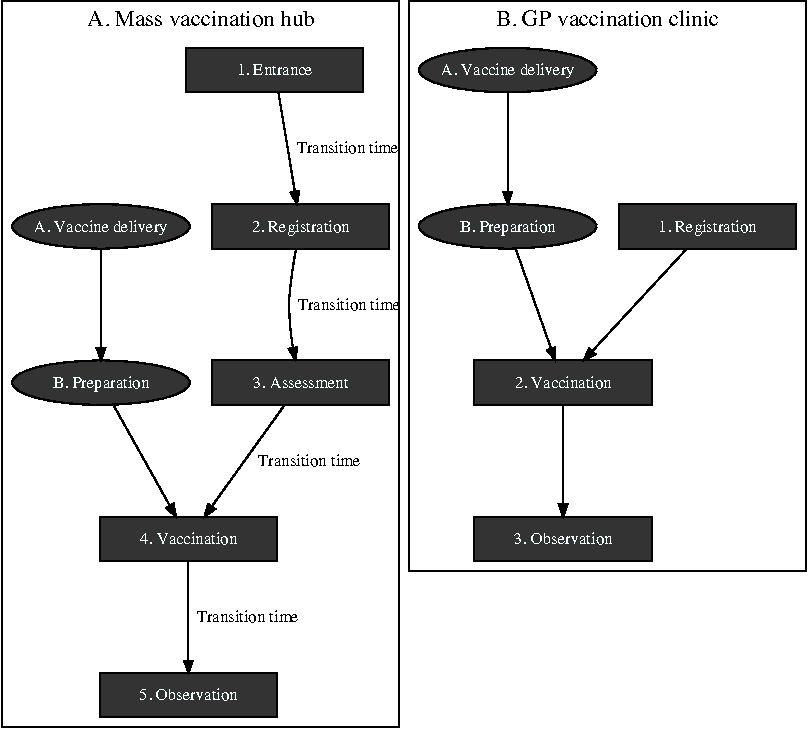
\includegraphics{Preprint_files/figure-latex/diagram-1} 

}

\caption{Queueing model for arena vaccination site (A) and GP vaccination site (B)}\label{fig:diagram}
\end{figure}

\hypertarget{queue-network-for-a-centralised-mass-vaccination-hub.}{%
\subsubsection{Queue network for a centralised mass vaccination
hub.}\label{queue-network-for-a-centralised-mass-vaccination-hub.}}

The proposed queue network for a mass vaccination hub is modelled on the
Phase 1a (Pfizer/BioNTech) vaccination hub based at the Royal Prince
Albert (RPA) hospital in Sydney. In this queue network, patients
traverse five stations: Entrance, Registration, Assessment, Vaccination
and Observation. The first four stations require the patient to wait for
an available staff member so these are modelled as queues, with new
arrivals serviced by the next available staff member on a
first-come-first-served basis. The observation stage does not require
patients to wait for an available staff member so this stage is modelled
as a stochastic lag period, with longer waits for a small proportion of
individuals to reflect adverse reactions. Because mass vaccination sites
require a large premises, the queue network also incorporates a short
transition time between stations.

Vaccine doses must be prepared close to the time they are administered,
and clearly delays to this process will result in delays at the
vaccination stage. To capture this feature of the vaccination process,
the queue network includes a parallel queue for vaccine preparation (see
Figure \ref{fig:diagram}A) which joins with the patient queue at the
vaccination station. The exact steps for the preparation process will
vary for the type of vaccine being administered.

\hypertarget{entrance}{%
\paragraph{1. Entrance:}\label{entrance}}

Patients arrive at the premises and queue up to get a temperature check
and to check-in to the venue. Hand sanitiser and masks are made
available. This station would be overseen by one or more health
professional staff but could also be supplemented with administrative
staff to help marshal patients to the next station.

\hypertarget{registration}{%
\paragraph{2. Registration:}\label{registration}}

Having passed through the entrance station, patients join the queue for
registration. The registration desks are staffed by one or more
personnel. As part of the registration process, patients will have their
current appointment confirmed and potentially could also book their
second vaccination. They are provided with pre-vaccination information
to read while they wait for the next station.

\hypertarget{assessment}{%
\paragraph{3. Assessment:}\label{assessment}}

Once registered, patients join the queue for assessment. The purpose of
assessment is to make sure that the patient is clinically suitable to
receive the vaccine. During this stage the patient's consent is also
recorded.

\hypertarget{vaccination}{%
\paragraph{4. Vaccination:}\label{vaccination}}

Having been given final clearance to receive the vaccine at the
assessment station, patients join the queue for vaccination. Once a
vaccinator becomes available, the patient can take a seat and expose
their upper arm. The vaccinator confirms the patients name and details
then administers the vaccine. The vaccinator applies a dressing to the
vaccination site, notes the vaccination time on a sticker and applies
this to the patient's shoulder or lapel.

\hypertarget{observation}{%
\paragraph{5. Observation:}\label{observation}}

Once vaccinated, patients advance to an observation area where they take
a seat and wait for the required time to ensure they experience no
immediate adverse reaction. A staff member will advise the patient once
their observation time has passed, at which point they can make their
way out of the premises.

\hypertarget{a.-vaccine-delivery}{%
\paragraph{A. Vaccine delivery:}\label{a.-vaccine-delivery}}

The proposed queue network does not set out to model vaccine delivery to
the vaccination site. All of our analyses assume that an adequate supply
of vaccine doses is available at the premises in the quantities required
to service all booked patients.

\hypertarget{b.-vaccine-preparation}{%
\paragraph{B. Vaccine preparation:}\label{b.-vaccine-preparation}}

Vaccines are delivered in multi-dose vials containing 5-6 doses (Pfizer)
or 8-10 doses (AstraZeneca). The exact preparation steps will differ
depending on the vaccine being prepared. Steps incorporated at this
station may include logging the vial, visual inspection of the dose,
reconstitution (for the Pfizer vaccine), and drawing the vaccine into
syringes.

\hypertarget{queue-network-for-a-local-gp-vaccination-clinic}{%
\subsubsection{Queue network for a local GP vaccination
clinic}\label{queue-network-for-a-local-gp-vaccination-clinic}}

The proposed queue network for a local GP vaccination clinic is
presented in Figure \ref{fig:diagram}B. In this queue network, patients
traverse three distinct stations: Registration, Vaccination and
Observation. To advance to the Registration and Vaccination stations,
patients must wait for the next available staff member so these stations
are modelled as queueing processes, with patients serviced by the next
available staff member on a first-come-first-served basis. As with the
mass vaccination model, the observation station is modelled as a
stochastic lag period rather than a queue, and there is a parallel queue
specified for vaccine preparation which joins at the vaccination
station. The time taken to walk between stations in a GP clinic is
assumed to be negligible and not included in the model. The distribution
of vaccination tasks across these stations is described in detail below.

\hypertarget{registration-1}{%
\paragraph{Registration:}\label{registration-1}}

Patients arrive at the premises, and receive a temperature check on
entry. They are provided with pre-vaccination information and a
check-list of contra-indicated items, either as a paper form or on a
hand-held tablet. While seated in a waiting area, they read the provided
information and complete the pre-vaccination checklist. Once complete,
they return the paper form or tablet to the staff member and wait for
the next available vaccinator. This process is assumed to take place in
a shared waiting area, which may also be used for the observation step.

\hypertarget{vaccination-1}{%
\paragraph{Vaccination:}\label{vaccination-1}}

Once a vaccinator becomes available, the patient advances to the
vaccination area, which may be a doctor's office or other suitable
partitioned area. The vaccinator reviews the patient's pre-vaccination
checklist, probes any items that have been checked and records the
patient's consent. The patient exposes their upper arm and the
vaccinator administers the vaccination and applies a dressing to the
vaccination site. Finally the vaccinator notes the vaccination time on a
sticker and applies this to the patients shoulder or lapel.

\hypertarget{observation-1}{%
\paragraph{Observation:}\label{observation-1}}

Once vaccinated, patients return to the waiting area where they take a
seat and wait for the allotted time to ensure they experience no adverse
reaction. The waiting area may be monitored by the same staff member who
is managing the registration process.

\hypertarget{assumed-service-times}{%
\subsection{Assumed service times}\label{assumed-service-times}}

For both the mass vaccination hub and GP vaccination clinic, the station
service times were modelled as exponential processes with fixed minimum
service times. Such exponential simulations reflect the typically
observed situation of most patients taking a relatively short time to
process, but with a ``long tail'' of some patients taking considerably
longer, and a few taking a very long time. The exception is the
observation station, which was modelled as bimodal distribution, with
normally distributed observation times for patients who did not
experience an adverse reaction and exponentially distributed observation
times for a small random subset to reflect a low incidence of adverse
reactions. The assumed minimum service times and exponential rate
parameters for each station are summarised in Table
\ref{tab:serviceTimeAssumptions}), together with the resulting
distribution of service times.

\begin{table}[!h]

\caption{\label{tab:serviceTimeAssumptions}Service time parameter values and resulting distributions}
\resizebox{\linewidth}{!}{
\begin{tabular}[t]{>{\raggedright\arraybackslash}p{4cm}>{\raggedright\arraybackslash}p{2cm}>{\raggedright\arraybackslash}p{2cm}>{\raggedleft\arraybackslash}p{1cm}>{\raggedleft\arraybackslash}p{1cm}>{\raggedleft\arraybackslash}p{1cm}>{\raggedleft\arraybackslash}p{1cm}>{\raggedleft\arraybackslash}p{1cm}>{}l}
\toprule
\multicolumn{3}{c}{ } & \multicolumn{5}{c}{Percentiles} & \multicolumn{1}{c}{ } \\
\cmidrule(l{3pt}r{3pt}){4-8}
Station & Form & Formula & 5\% & 25\% & 50\% & 75\% & 95\% & Distribution\\
\midrule
\addlinespace[0.3em]
\multicolumn{9}{l}{\textbf{Arena model}}\\
\cellcolor{gray!6}{Preparation} & \cellcolor{gray!6}{exponential} & \cellcolor{gray!6}{1 + exp(3)} & \cellcolor{gray!6}{1.0} & \cellcolor{gray!6}{1.1} & \cellcolor{gray!6}{1.2} & \cellcolor{gray!6}{1.4} & \cellcolor{gray!6}{2.0} & \cellcolor{gray!6}{
\includegraphics[width=0.67in, height=0.17in]{Preprint_files/figure-latex//hist_1af9480384b6.pdf}}\\
Entrance & exponential & 2 + exp(1) & 2.0 & 2.3 & 2.7 & 3.4 & 5.4 & 
\includegraphics[width=0.67in, height=0.17in]{Preprint_files/figure-latex//hist_1af970fe22f7.pdf}\\
\cellcolor{gray!6}{Registration} & \cellcolor{gray!6}{exponential} & \cellcolor{gray!6}{3 + exp(0.7)} & \cellcolor{gray!6}{3.1} & \cellcolor{gray!6}{3.4} & \cellcolor{gray!6}{4.0} & \cellcolor{gray!6}{5.0} & \cellcolor{gray!6}{7.4} & \cellcolor{gray!6}{
\includegraphics[width=0.67in, height=0.17in]{Preprint_files/figure-latex//hist_1af92c81c1d0.pdf}}\\
Assessment & exponential & 2 + exp(1) & 2.0 & 2.3 & 2.6 & 3.3 & 4.7 & 
\includegraphics[width=0.67in, height=0.17in]{Preprint_files/figure-latex//hist_1af955cb4a78.pdf}\\
\cellcolor{gray!6}{Vaccination} & \cellcolor{gray!6}{exponential} & \cellcolor{gray!6}{3 + exp(1)} & \cellcolor{gray!6}{3.1} & \cellcolor{gray!6}{3.3} & \cellcolor{gray!6}{3.7} & \cellcolor{gray!6}{4.3} & \cellcolor{gray!6}{5.9} & \cellcolor{gray!6}{
\includegraphics[width=0.67in, height=0.17in]{Preprint_files/figure-latex//hist_1af91ed94ba9.pdf}}\\
Observation & normal & norm(20, 0.5) & 19.8 & 19.9 & 20.0 & 20.1 & 20.2 & 
\includegraphics[width=0.67in, height=0.17in]{Preprint_files/figure-latex//hist_1af919094f0d.pdf}\\
\cellcolor{gray!6}{Adverse reaction} & \cellcolor{gray!6}{exponential} & \cellcolor{gray!6}{20 + exp(0.1)} & \cellcolor{gray!6}{20.5} & \cellcolor{gray!6}{22.8} & \cellcolor{gray!6}{27.0} & \cellcolor{gray!6}{33.9} & \cellcolor{gray!6}{50.6} & \cellcolor{gray!6}{
\includegraphics[width=0.67in, height=0.17in]{Preprint_files/figure-latex//hist_1af915d56e36.pdf}}\\
\addlinespace[0.3em]
\multicolumn{9}{l}{\textbf{GP model}}\\
Preparation & exponential & 1 + exp(2) & 1.0 & 1.1 & 1.2 & 1.4 & 2.0 & 
\includegraphics[width=0.67in, height=0.17in]{Preprint_files/figure-latex//hist_1af96ce8357e.pdf}\\
\cellcolor{gray!6}{Registration} & \cellcolor{gray!6}{exponential} & \cellcolor{gray!6}{1 + exp(3)} & \cellcolor{gray!6}{3.1} & \cellcolor{gray!6}{3.3} & \cellcolor{gray!6}{3.8} & \cellcolor{gray!6}{4.5} & \cellcolor{gray!6}{6.1} & \cellcolor{gray!6}{
\includegraphics[width=0.67in, height=0.17in]{Preprint_files/figure-latex//hist_1af9486034ad.pdf}}\\
Vaccination & exponential & 1 + exp(3) & 5.1 & 5.6 & 6.5 & 7.7 & 11.1 & 
\includegraphics[width=0.67in, height=0.17in]{Preprint_files/figure-latex//hist_1af950a3f19e.pdf}\\
\cellcolor{gray!6}{Observation} & \cellcolor{gray!6}{normal} & \cellcolor{gray!6}{norm(20, 0.5)} & \cellcolor{gray!6}{19.2} & \cellcolor{gray!6}{19.7} & \cellcolor{gray!6}{20.0} & \cellcolor{gray!6}{20.3} & \cellcolor{gray!6}{20.8} & \cellcolor{gray!6}{
\includegraphics[width=0.67in, height=0.17in]{Preprint_files/figure-latex//hist_1af973c3b72b.pdf}}\\
Adverse reaction & exponential & 20 + exp(0.1) & 20.5 & 22.6 & 26.4 & 33.1 & 48.8 & 
\includegraphics[width=0.67in, height=0.17in]{Preprint_files/figure-latex//hist_1af92feb64e5.pdf}\\
\bottomrule
\end{tabular}}
\end{table}

\hypertarget{assumed-arrival-times}{%
\subsection{Assumed arrival times}\label{assumed-arrival-times}}

Arrivals for both queue networks were based on fixed appointment slots
across an eight hour clinic running from 8am to 4pm. For mass
vaccination hubs we assumed that appointment arrival times would be
given on the hour, every hour. For local GP hubs we assumed that
appointment slots would be provided in ten minute intervals. Actual
arrival times were based on the appointment schedule with the addition
of some random noise, reflecting that most people would turn up somewhat
before their allotted time, while a smaller proportion would arrive
after their allotted time. Arrival times also accounted for a small
proportion of no-shows, set at 2\% for both local and mass vaccination
hubs. The actual number of arrivals per appointment interval was
calibrated to keep the queue performance metrics within reasonable
limits. As an example, Figure \ref{fig:arrivalTimes} presents simulated
arrival times for a mass vaccination hub at the rate of 120 arrivals
every hour, and a GP vaccination clinic at a rate of 4 arrivals every 10
minutes.

\begin{figure}

{\centering 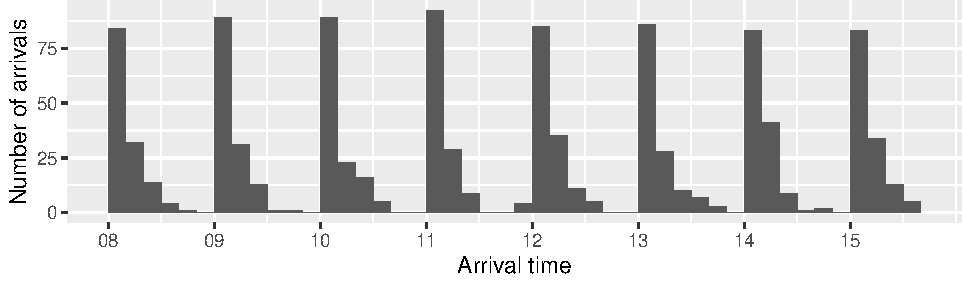
\includegraphics{Preprint_files/figure-latex/arrivalTimes-1} 

}

\caption{Randomly generated arrival times for a mass vaccination hub (A) and a GP vaccination clinic (B)}\label{fig:arrivalTimes}
\end{figure}

\hypertarget{staffing-levels}{%
\subsection{Staffing levels}\label{staffing-levels}}

For each of the proposed queue networks we specified models with low,
medium and high staffing availability, ranging from 21 to 63 healthcare
staff for mass vaccination sites and from 4 to 12 healthcare staff for
GP vaccination clinics (Table \ref{tab:staffing}). The distribution of
staff across the stations of the queue network was kept stable
regardless of the total staffing capacity. For example, for the mass
vaccination model there were three staff assigned to the Registration
station for every one staff member assigned to the Preparation station,
regardless of the assumed size of the hub. This equivalence facilitated
valid comparisons across hub sizes presented later in the analysis.

\begin{table}[!h]

\caption{\label{tab:staffing}Staff numbers by station for low, medium and high staffing availability}
\resizebox{\linewidth}{!}{
\begin{tabular}[t]{>{\raggedright\arraybackslash}p{2cm}>{\raggedleft\arraybackslash}p{2cm}>{\raggedleft\arraybackslash}p{2cm}>{\raggedleft\arraybackslash}p{2cm}>{\raggedleft\arraybackslash}p{2cm}>{\raggedleft\arraybackslash}p{2cm}>{\raggedleft\arraybackslash}p{2cm}}
\toprule
\multicolumn{1}{c}{ } & \multicolumn{6}{c}{Staff numbers} \\
\cmidrule(l{3pt}r{3pt}){2-7}
Size & Preparation & Entrance & Registration & Assessment & Vaccination & Total\\
\midrule
\addlinespace[0.3em]
\multicolumn{7}{l}{\textbf{Mass vaccination hub}}\\
\cellcolor{gray!6}{low} & \cellcolor{gray!6}{2} & \cellcolor{gray!6}{4} & \cellcolor{gray!6}{6} & \cellcolor{gray!6}{4} & \cellcolor{gray!6}{5} & \cellcolor{gray!6}{21}\\
medium & 4 & 8 & 12 & 8 & 10 & 42\\
\cellcolor{gray!6}{high} & \cellcolor{gray!6}{6} & \cellcolor{gray!6}{12} & \cellcolor{gray!6}{18} & \cellcolor{gray!6}{12} & \cellcolor{gray!6}{15} & \cellcolor{gray!6}{63}\\
\addlinespace[0.3em]
\multicolumn{7}{l}{\textbf{Local GP hub}}\\
low & 1 & * & 1 & * & 2 & 4\\
\cellcolor{gray!6}{medium} & \cellcolor{gray!6}{2} & \cellcolor{gray!6}{*} & \cellcolor{gray!6}{2} & \cellcolor{gray!6}{*} & \cellcolor{gray!6}{4} & \cellcolor{gray!6}{8}\\
high & 3 & * & 3 & * & 6 & 12\\
\bottomrule
\multicolumn{7}{l}{\rule{0pt}{1em}\textsuperscript{*} Not applicable}\\
\end{tabular}}
\end{table}

Note that the total staffing numbers given in Table \ref{tab:staffing}
only include staffing requirements for the stations in the assumed queue
network that imply a queueing process and do not cover all staffing
needs to successfully run a vaccination clinic. For example, the staff
needed to oversee the observation station are not included because
patients do not have to queue up to be serviced at this station. Also
not included here are other support staff, such as supervisors,
cleaners, marshals and caterers. The number and type of support staff
required will vary depending on the size of the vaccination hub, and
must also be taken into account when planning vaccine distribution.

\hypertarget{queue-performance}{%
\subsection{Queue performance}\label{queue-performance}}

We use two metrics to quantify queue performance, total processing time
and staff utilisation. Total processing time, measured here in minutes,
is the total time from start to finish of the queue network. Staff
utilisation is the average proportion of staff that are busy across the
simulation run. An established property of queueing models is that queue
performance rapidly degrades as staff utilisation exceeds
80\%.{[}little1961proof{]}

\hypertarget{software-and-code}{%
\subsection{Software and code}\label{software-and-code}}

The analysis was performed using R version 4.0.3\textsuperscript{15} and
associated packages.\textsuperscript{16} Queueing models were simulated
using the \texttt{queuecomputer} package.{[}ebert2017computationally{]}
The complete source code to reproduce this analysis can be accessed at
\url{https://github.com/CBDRH/vaccineQueueNetworks}.

\hypertarget{results}{%
\section{Results}\label{results}}

\hypertarget{calibrating-arrivals-to-achieve-reasonable-service-times-and-staff-utilisation}{%
\subsection{Calibrating arrivals to achieve reasonable service times and
staff
utilisation}\label{calibrating-arrivals-to-achieve-reasonable-service-times-and-staff-utilisation}}

In this section we present estimates of median processing times and
average staff utilisation based on (i) the queue networks presented in
Figure \ref{fig:diagram} and (ii) the stochastic service times described
in Table \ref{tab:serviceTimeAssumptions}. The number of available staff
(and thus the number of open queues) at each station is fixed to be
constant at the levels set out in Table \ref{tab:staffing}. Within each
setting, the frequency of arrivals is increased gradually. For example,
for the mass vaccination site with low staffing numbers, the frequency
of arrivals was increased from 10 per hour to 110 per hour, in
increments of 25. For each of the six resulting models, the average
processing time and staff utilisation across 20 simulation runs are
presented in Figure \ref{fig:processingTimes} and
\ref{fig:staffUtilisation} respectively.

\begin{figure}

{\centering 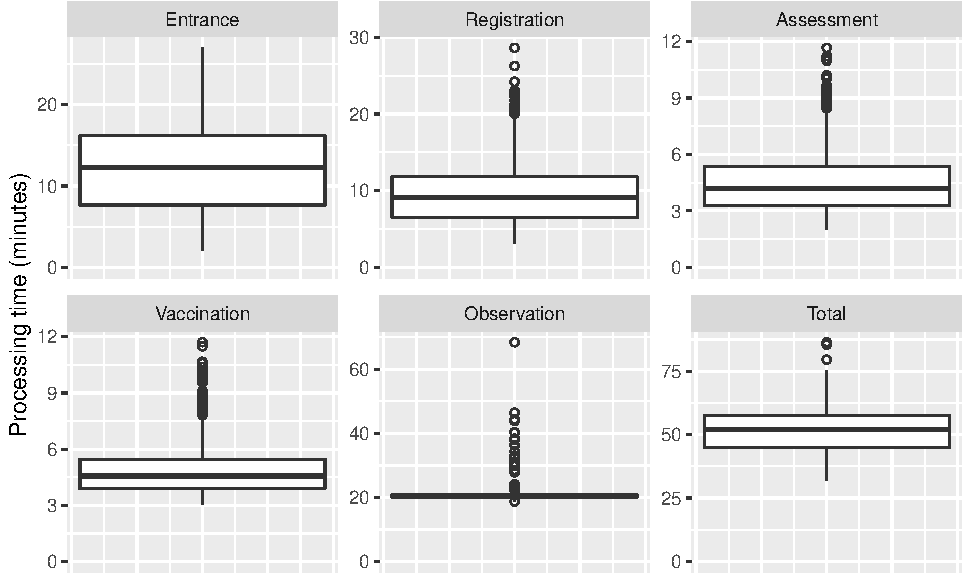
\includegraphics{Preprint_files/figure-latex/processingTimes-1} 

}

\caption{Median processing times by arrival frequency for a mass vaccination hub (A) and a GP vaccination clinic (B)}\label{fig:processingTimes}
\end{figure}

Figure \ref{fig:processingTimes} presents the median processing time as
the arrival frequency increases. When arrivals are set to their lowest
value, all processing times are within between 30 and 60 minutes (the
shaded band). In general, small increases to the average arrival rate
have a negligible impact on the overall median processing time. However,
once a certain threshold is reached, the median processing time quickly
escalates. For both mass vaccination hubs and GP vaccination clinics,
the critical threshold is lower in venues with relatively low staffing
and higher in venues with relatively high staffing, a point we will
return to later.

Figure \ref{fig:staffUtilisation} presents the corresponding arithmetic
mean staff utilisation for the Vaccination station, which was chosen as
an example because it is common to both the mass vaccination hub and the
GP vaccination clinic. Utilisation for the other stations are not
presented but display similar patterns.

\begin{figure}

{\centering 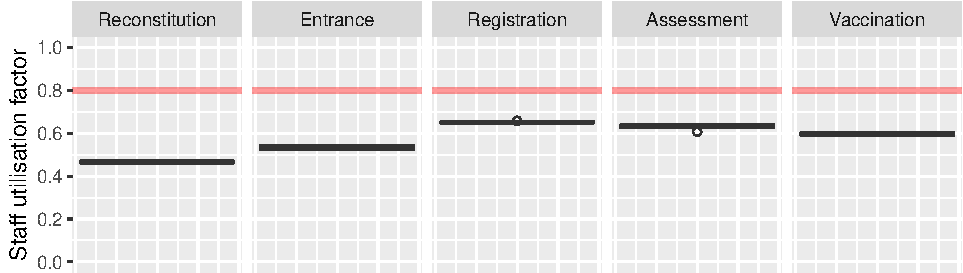
\includegraphics{Preprint_files/figure-latex/staffUtilisation-1} 

}

\caption{Average staff utilisation by arrival frequency for a mass vaccination hub (A) and a GP vaccination clinic (B)}\label{fig:staffUtilisation}
\end{figure}

As the arrival frequency increases, mean staff utilisation grows
gradually. The shaded area indicates a staff utilisation factor between
0.5 and 0.7. Beyond this level, mean utilisation rapidly increases as
arrivals increase.

These results emphasise the delicate balance between arrival frequency,
mean staff utilisation and processing times. If arrivals are two low,
processing times will be at an acceptable level but the available staff
will be under-utilised. As arrivals increase, processing times and staff
utilisation increase accordingly. However if the rate of arrivals grows
too high, mean staff utilisation passes a critical threshold and
processing times expand beyond reasonable levels.

Based on this calibration exercise, we specified the number of arrivals
such that the median processing times remained under an hour, and the
staff utilisation did not exceed 0.7 for any station. The chosen arrival
frequencies that met this criteria are presented in Table
\ref{tab:arrivalFreq}.

\begin{table}[!h]

\caption{\label{tab:arrivalFreq}Arrival frequency by station for low, medium and high staffing availability}
\centering
\begin{tabular}[t]{>{\raggedright\arraybackslash}p{4cm}>{\raggedleft\arraybackslash}p{2cm}>{\raggedleft\arraybackslash}p{2cm}}
\toprule
Size & Appointment interval & Arrivals per interval\\
\midrule
\addlinespace[0.3em]
\multicolumn{3}{l}{\textbf{Mass vaccination hub}}\\
\cellcolor{gray!6}{low} & \cellcolor{gray!6}{60 minutes} & \cellcolor{gray!6}{60}\\
medium & 60 minutes & 120\\
\cellcolor{gray!6}{high} & \cellcolor{gray!6}{60 minutes} & \cellcolor{gray!6}{180}\\
\addlinespace[0.3em]
\multicolumn{3}{l}{\textbf{GP vaccination clinic}}\\
low & 10 minutes & 2\\
\cellcolor{gray!6}{medium} & \cellcolor{gray!6}{10 minutes} & \cellcolor{gray!6}{4}\\
high & 10 minutes & 6\\
\bottomrule
\end{tabular}
\end{table}

The chosen arrival frequencies were selected to increase linearly across
the low, medium and high staffing models: arrivals for the mass
vaccination hub were set at 60, 120 and 180 arrivals per hour at
relatively low, medium and high staffed hubs; arrivals for GP clinics
were set at 2, 4, and 6 arrivals per 10 minutes. Scaling the arrivals
and staffing in this way ensured that the baseline staff utilisation and
processing times remained constant across all models within the given
queue network (see Figure \ref{fig:baselineUtilisation} and Figure
\ref{fig:baselineProcessingTimes}). This equivalence facilitates
comparisons between hub sizes within the two queue networks.

\begin{figure}

{\centering 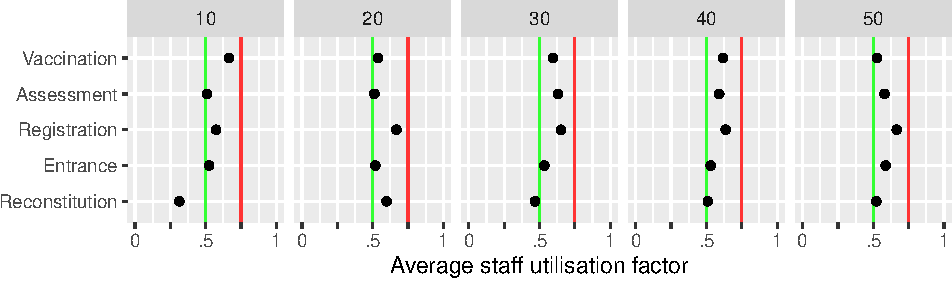
\includegraphics{Preprint_files/figure-latex/baselineUtilisation-1} 

}

\caption{Baseline staff utilisation factor for mass vaccination hubs (A) and GP vaccination clinics (B)}\label{fig:baselineUtilisation}
\end{figure}

\begin{figure}

{\centering 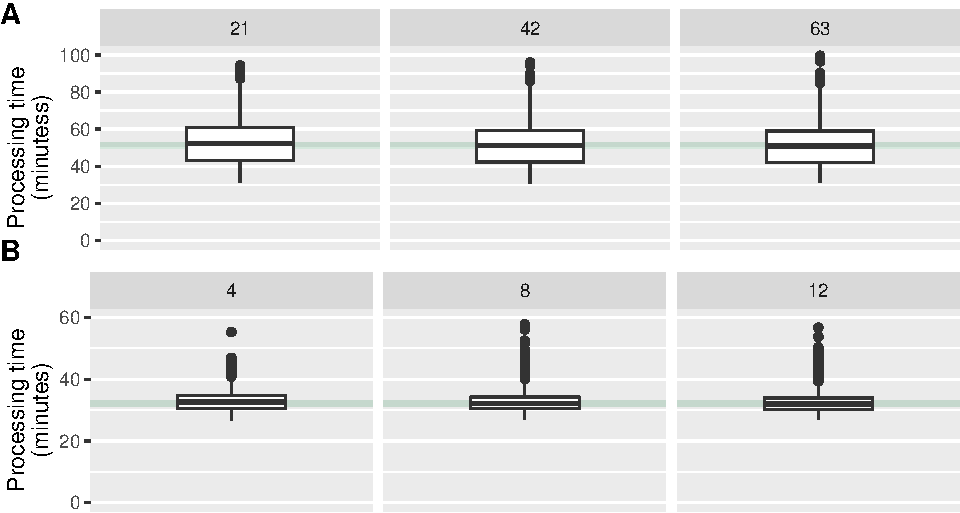
\includegraphics{Preprint_files/figure-latex/baselineProcessingTimes-1} 

}

\caption{Baseline median processing times for the mass vaccination hub (A) and GP vaccination clinic (B)}\label{fig:baselineProcessingTimes}
\end{figure}

The results in Figures \ref{fig:baselineUtilisation} and
\ref{fig:baselineProcessingTimes} illustrate that for both the mass
vaccination hubs and GP clinic baseline models, the staff utilisation
and processing times are stable regardless of the staffing capacity.
This equivalence is important for the stress tests reported below,
because it means the different models are starting from the same
baseline in terms of queue performance.

\hypertarget{daily-throughput}{%
\subsection{Daily throughput}\label{daily-throughput}}

Based on the calibrated baseline models, we can now estimate the number
of daily vaccinations possible at different site capacities while
maintaining processing times and staff utilisation within reasonable
limits. The results are presented in Figure
\ref{fig:baselineThroughput}.

\begin{figure}

{\centering 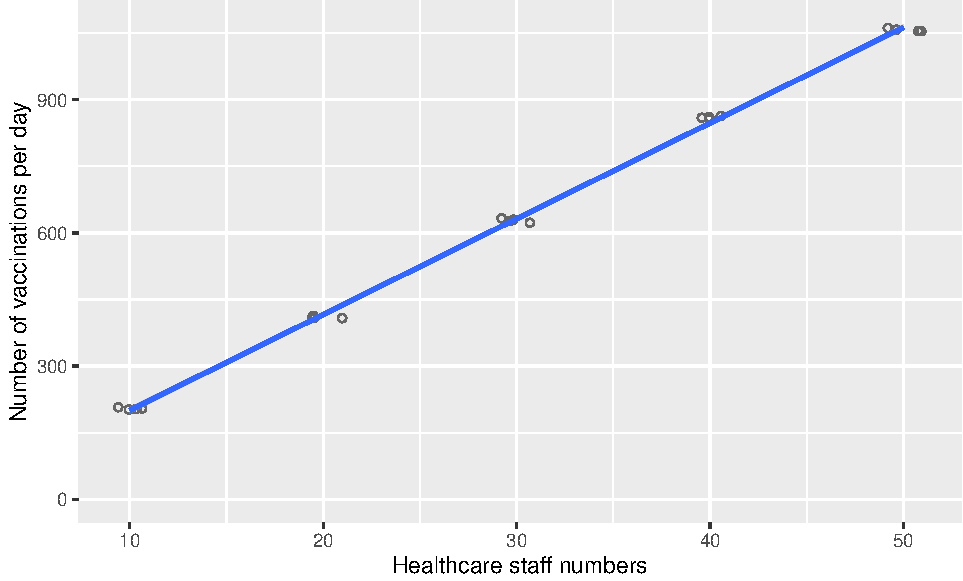
\includegraphics{Preprint_files/figure-latex/baselineThroughput-1} 

}

\caption{Baseline daily throughput for mass vaccination hubs (A) and GP vaccination clinics (B)}\label{fig:baselineThroughput}
\end{figure}

The results show that, while holding queue performance metrics constant,
the number of daily vaccinations scales linearly with increasing
healthcare staff for both the mass vaccination hub and GP vaccination
clinic. The potential daily throughput for an eight hour clinic at a
mass vaccination hub ranged from around 500 vaccinations for a
relatively small hub to 1,400 vaccinations a day for a relatively large
hub. For GP vaccination clinics, the estimated daily throughput ranged
from about 100 vaccinations a day for a relatively small practice to
almost 300 a day for a relatively large practice.

\hypertarget{stress-tests}{%
\subsection{Stress tests}\label{stress-tests}}

In this section, we apply two stress tests to our baseline models. The
first test was to gradually increase arrivals, which could reflect
efforts to increase throughput with the same staffing levels. This could
arise if the production of vaccine doses increased or there were other
imperatives, such as a large-scale COVID-19 outbreak. The second stress
test was to gradually decrease staff numbers, which could reflect
inevitable fluctuations in staff availability due to illness etc, or
healthcare staff having to attend to a medical emergencies or routine
duties.

\hypertarget{increasing-arrivals}{%
\subsubsection{Increasing arrivals}\label{increasing-arrivals}}

Figure \ref{fig:processingTimeTest} presents the median processing time
based on incrementing the arrival frequency from the levels set for the
baseline models. For mass vaccination hubs and GP clinics, increasing
the number of arrivals results in increased processing times. However,
the rate of increase in processing times is larger for sites with
relatively low healthcare staff compared to sites with relatively high
healthcare staffing.

\begin{figure}

{\centering 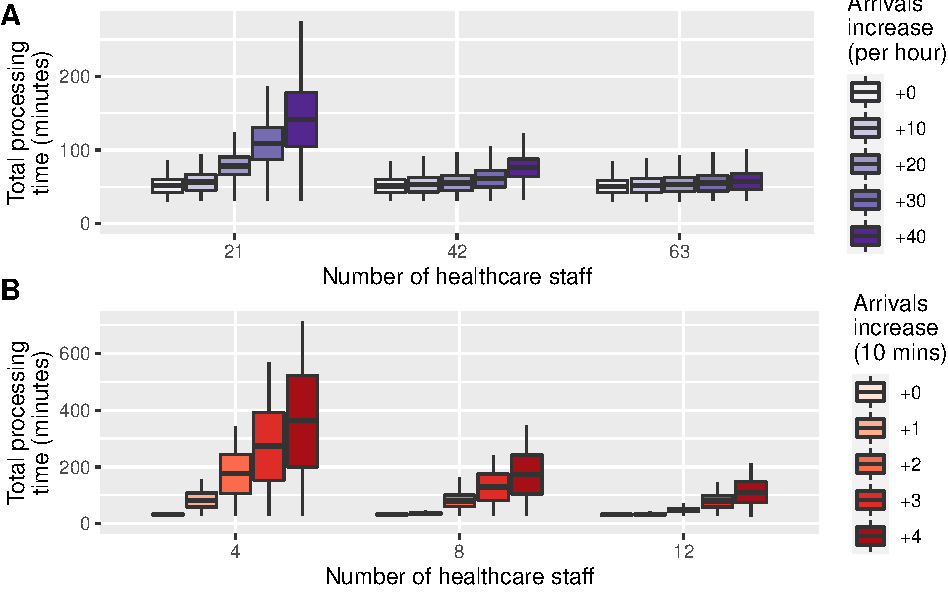
\includegraphics{Preprint_files/figure-latex/processingTimeTest-1} 

}

\caption{Increase in processing time with increased arrivals by site size for mass vaccination hubs (A) and GP vaccination clinics (B)}\label{fig:processingTimeTest}
\end{figure}

\begin{figure}

{\centering 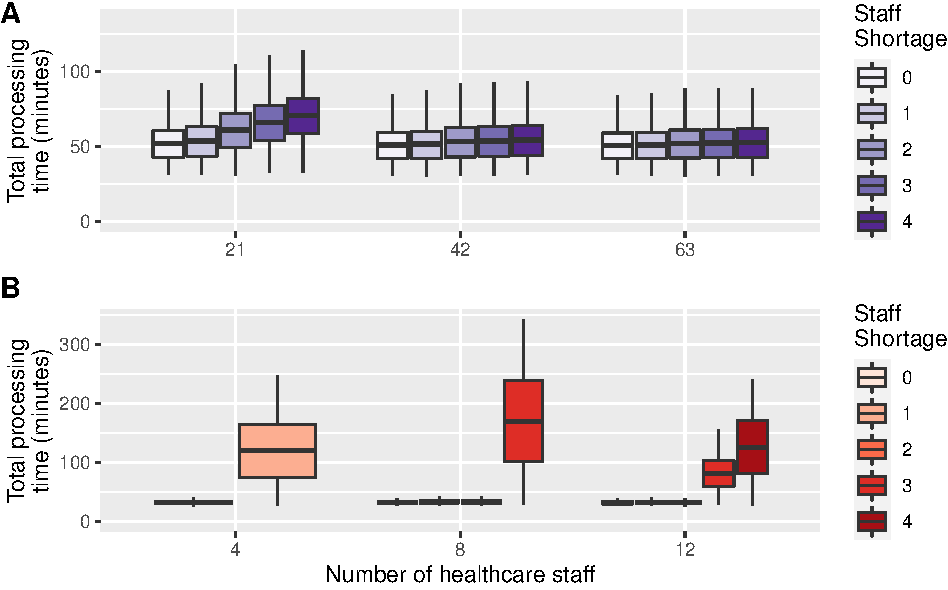
\includegraphics{Preprint_files/figure-latex/staffShortageTest-1} 

}

\caption{Increase in processing time with staff shortages by site size}\label{fig:staffShortageTest}
\end{figure}

\hypertarget{staff-shortages}{%
\subsubsection{Staff shortages}\label{staff-shortages}}

Figure \ref{fig:staffShortageTest} presents the average processing time
based on gradually decreasing the available staff for a given model.
These results show that---unsurprisingly---small vaccination sites with
limited staff numbers are quickly affected by staff shortages, whereas
large vaccination hubs with more staff can still maintain queue
performance with the same number of staff shortages.

\hypertarget{interactive-web-based-queue-simulation-applet}{%
\section{Interactive web-based queue simulation
applet}\label{interactive-web-based-queue-simulation-applet}}

To accompany the analysis presented here, we have developed an
interactive web-based queue simulation applet. This applet provides a
graphical user interface to the mass vaccination and GP clinic queueing
networks estimated with the R package \texttt{queuecomputer}. On
launching the applet, the results from two default models are presented.
These models have been parameterised to reflect the medium-sized
baseline model presented here, i.e.~the mass vaccination centre with 42
staff members and the GP clinic with eight staff members. The
interactive interface allows users to adjust the assumed arrival times,
service times and available staff to reflect their own situation or
assumptions. Queue performance is summarised in terms of total
throughput, processing times and staff utilisation (Figure
\ref{fig:shinyScreenshot}).

\begin{figure}

{\centering 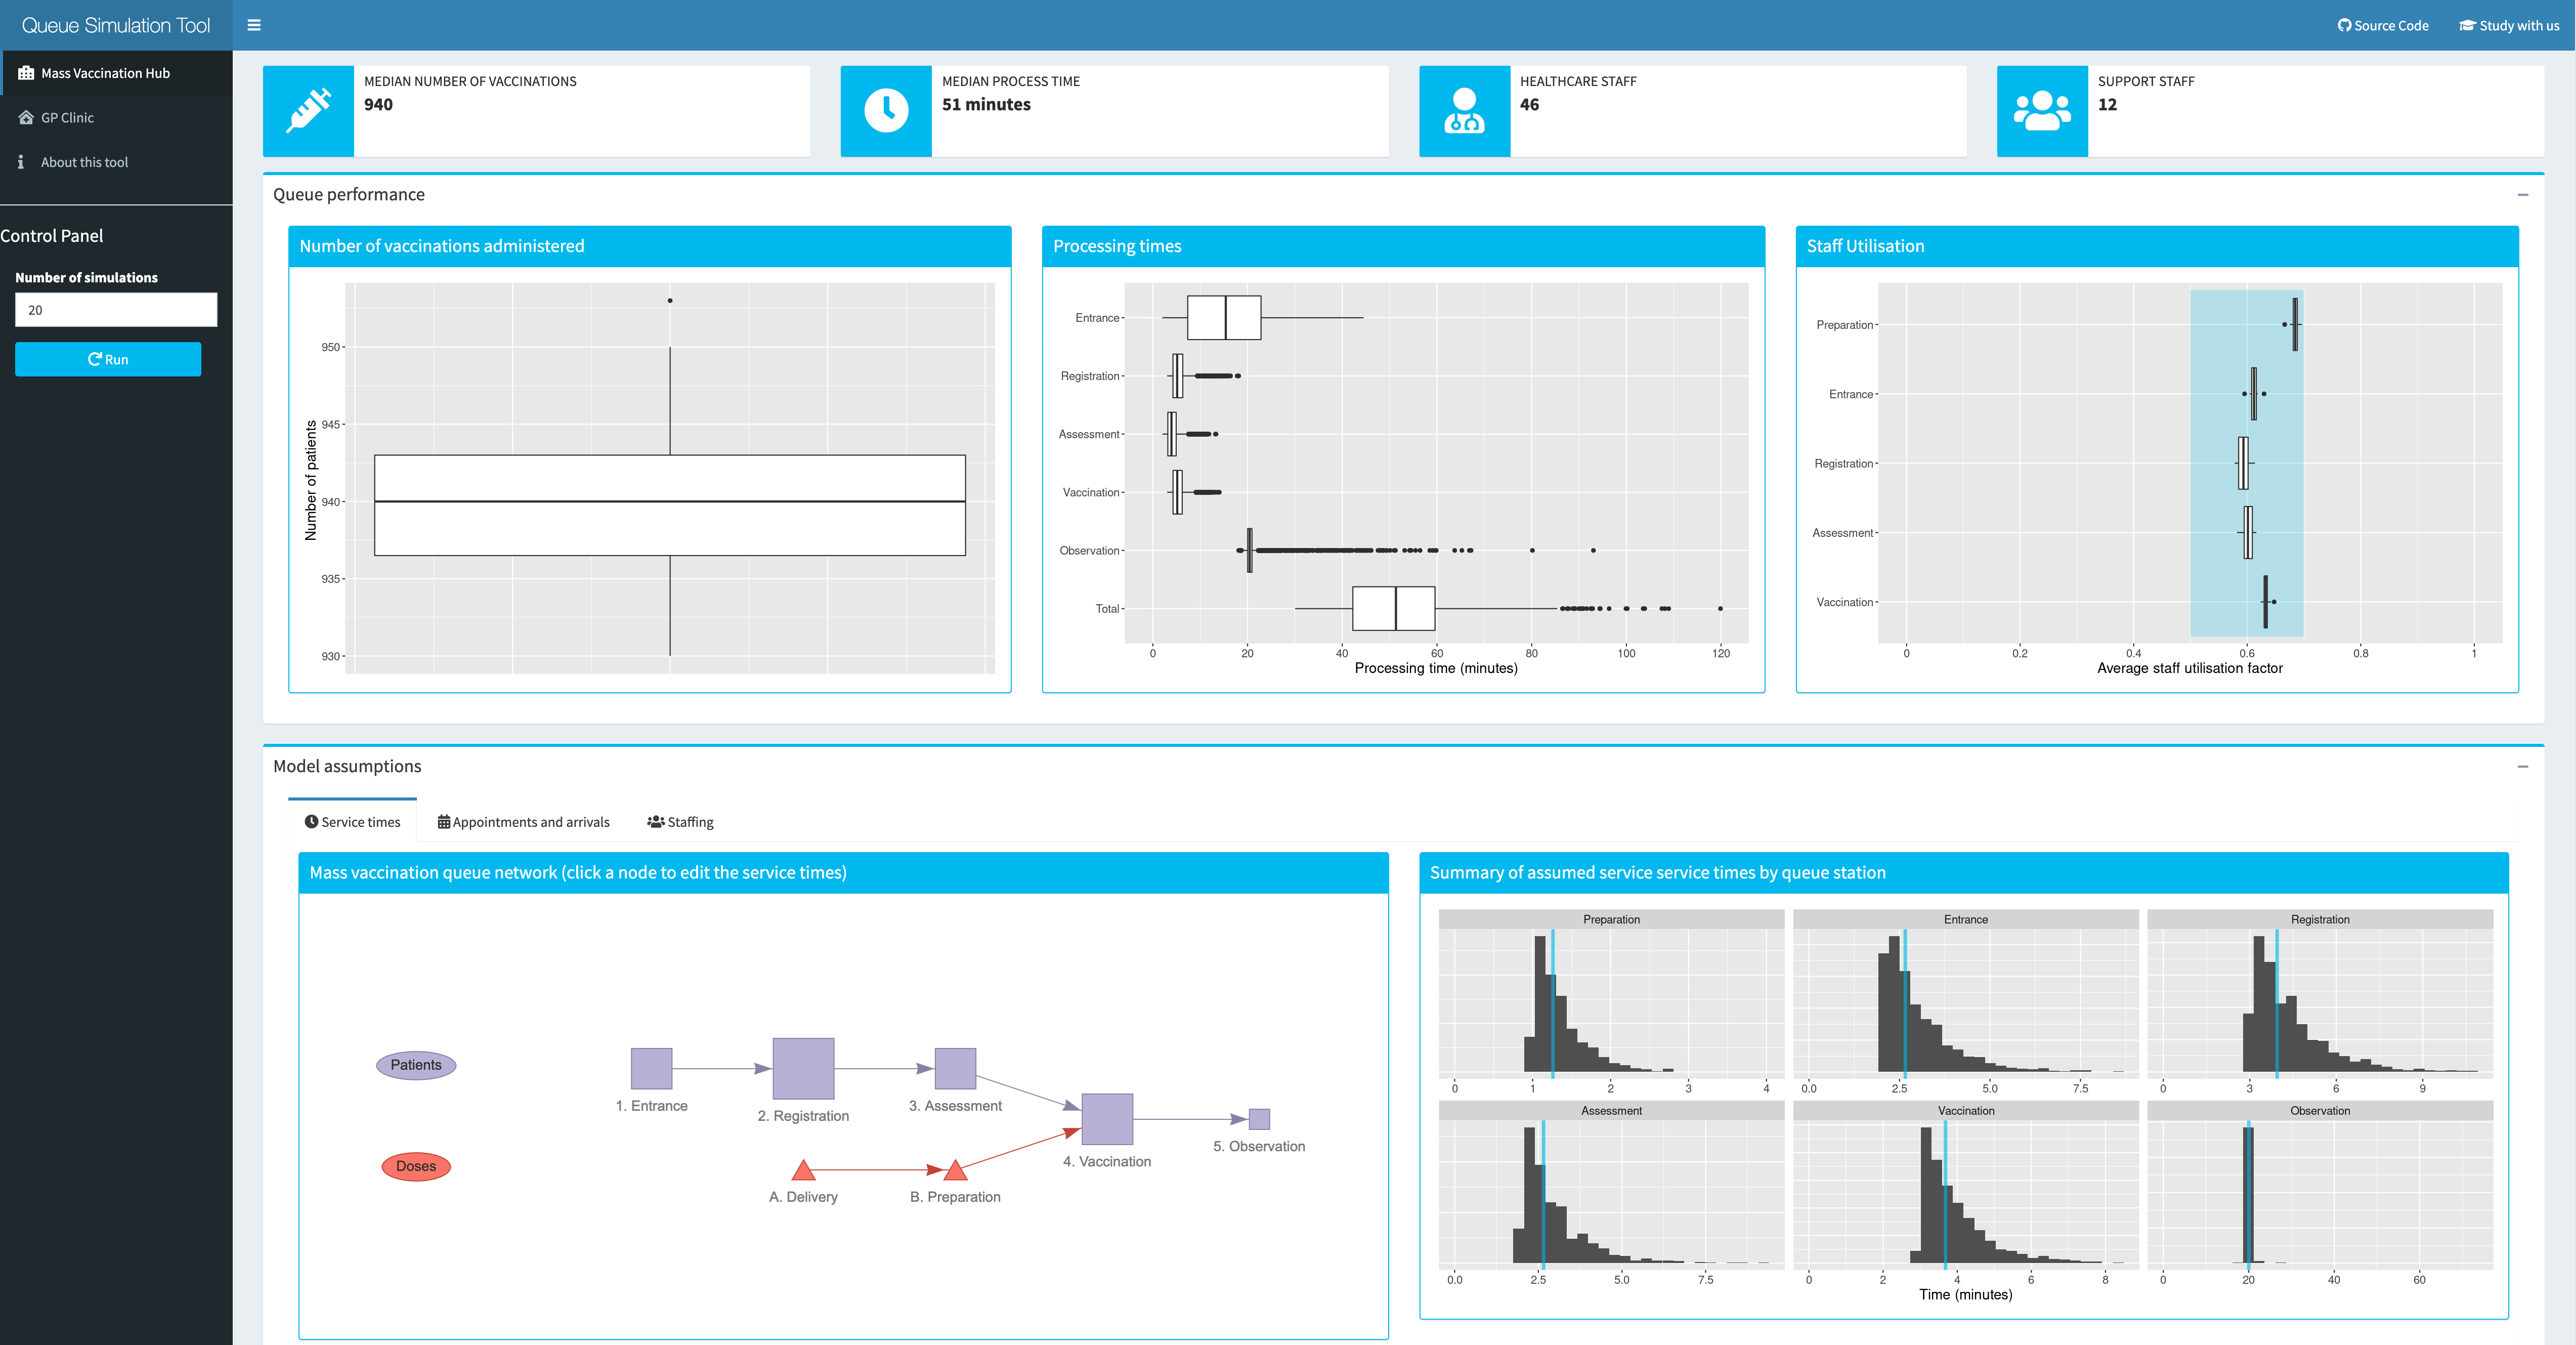
\includegraphics[width=5.09in]{../Data/queue-sim-tool-screenshot} 

}

\caption{Screenshot of the interactive web-based queue simulation applet}\label{fig:shinyScreenshot}
\end{figure}

The applet can be accessed at \url{https://cbdrh.shinyapps.io/queueSim}.
The underlying source code is available on GitHub here:
\url{https://github.com/CBDRH/vaccineQueueNetworks}. Planned extensions
of this applet will allow users to download a summary of their specified
assumptions and queue perfromance metrics, as well as the underlying
simulation data.

\hypertarget{discussion}{%
\section{Discussion}\label{discussion}}

\hypertarget{summary-and-discussion-of-main-results}{%
\subsection{Summary and discussion of main
results}\label{summary-and-discussion-of-main-results}}

We have used queueing simulation methods to model the vaccination
process based on two modes of delivery: a large mass vaccination hub and
a small GP vaccination clinic. For each delivery mode, we calibrated the
number of arrivals that could be vaccinated over an eight hour period
while keeping two queue performance measures---staff utilisation and
total processing time---constrained to reasonable levels. Our results
provide estimates of potential daily throughput for these distinct
vaccine delivery modes across a range of staffing levels. Under our
assumed service times, a relatively small GP clinic could perform around
100 vaccinations over an eight-hour clinic, while a relatively large
mass vaccination hub could perform around 1,400 vaccinations over the
same time period. Put differently, one large mass vaccination hub can
achieve the same coverage as 14 GP small vaccination clinics.

These throughput estimates have reasonable face-validity. The mass
vaccination hub trialled by NSW Health in a 2008 pandemic response
planning exercise administered 498 vaccines in five hours using a mass
vaccination process delivered through a local
school.\textsuperscript{12} The RPA Pfizer clinic has been delivering
between 1,100 and 1,400 vaccinations per day throughout March 2021.

Our models suggest that daily vaccination capacity scales linearly with
staffing capacity while maintaining a constant queue performance.
However, there are several other facets of the vaccine delivery process
that are likely to offer economies-of-scale. For example, given a low
incidence of adverse events, a high-capacity post-vaccination area
observation area could be overseen by a single staff member.
Economies-of-scale area are also likely to apply to vaccine delivery,
because it may be logistically more efficient and cost-effective to
coordinate a single delivery to one centralised hub rather than multiple
deliveries to numerous smaller clinics.

By stressing our baseline models, we have shown that mass vaccination
hubs are better placed to scale up daily throughput with a fixed staff
capacity while maintaining acceptable queue performance. We have also
shown that mass vaccination hubs are also are more resilient to staff
shortages.

\hypertarget{policy-implications}{%
\subsection{Policy implications}\label{policy-implications}}

To date, the Australian Government's approach to vaccine delivery has
relied on hospital hubs, private contractors and the Australian Defence
Forces to administer the Pfizer Vaccine to the highest priority phase,
whereas delivery of subsequent phases is planned through smaller sites,
including general practices, Aboriginal Controlled Community Health
Services, and community pharmacies, to administer the AstraZeneca
vaccine to the bulk of the Australian population. There has been little
emphasis on the use of mass vaccination hubs to be included in
vaccination efforts, although previous pandemic planning exercises found
this model to be effective,\textsuperscript{12} and mass vaccination
sites have been implemented successfully in Australia (during Phase 1a
of the COVID-19 vaccine roll-out) and overseas.\textsuperscript{17,18}

Mass vaccination hubs and GP clinics offer distinct advantages as modes
of vaccine delivery. As we have shown, mass vaccination hubs are more
robust to increased throughput and staff shortages. Smaller GPs and CPs
are more likely to be vulnerable to concomitant workplace demands, which
fluctuate during the year and increase notably during the winter months.
GPs have the advantage of existing infrastructure and existing
relationships with patients. GPs are also highly flexible and can adapt
to specific needs local circumstances and specific needs, as seen with
carpark drive-through testing sites, which many practices set up during
the COVID-19 pandemic.\textsuperscript{19} The optimal vaccination site
may vary for different population segments. Older people or clinically
vulnerable patients may benefit from attending their local GP who will
be familiar with their medical history. Younger working adults may
benefit from extended hours or more flexible appointment scheduling that
could be offered by a mass vaccination hub. It may be easiest to reach
university students, and in due course younger children, through
vaccination hubs set up in campuses and schools.

Expanding GP capacity to vaccinate and supporting practices to offer
more flexible models for vaccination will assist in achieving
Australia's mass vaccination goals. Other vaccination delivery modes
such as adapting drive-through mass testing sites should also be
explored. A combination of expanded mass vaccination hubs and expanded
GP vaccination is likely to achieve mass vaccination faster than either
alone.

\hypertarget{limitations}{%
\subsection{Limitations}\label{limitations}}

An obvious limitation of our analysis is that the queueing models assume
sufficiently available vaccine doses. We have not attempted to model the
process of vaccine procurement or the logistics of delivering vaccine
doses to the venues where they will of administered. Our analysis does
not account for essential staff who are not involved in the queueing
process but do need to be considered when estimating staffing
requirements. The assumed queue networks rely on subjective assumptions
of the distribution of service times at each station. We specified
service times that had reasonable face-validity and produced realistic
estimates of overall processing times. This could be further improved in
the future through a time-use survey to empirically estimate service
time distributions for each station in a queue network. Our web-based
queueing simulation applet allows queue performance to be explored under
different sets of assumptions for service times, appointment schedules
and staffing availability.

\hypertarget{conclusion}{%
\subsection{Conclusion}\label{conclusion}}

Stochastic queueing models can be used to simulate vaccination queues,
estimate daily throughput based on given staff availability and inform
service delivery. Different modes of vaccine distribution have different
benefits and challenges. Mass vaccination clinics offer a higher daily
throughput and are more resilient to increased arrivals and decreased
staff availability, however they require larger premises and higher
staffing numbers. GP vaccination clinics can perform vaccinations at a
similar rate per staff member compared to mass vaccination hubs, however
it may be difficult to sustain a high throughput given existing
workloads and incomplete coverage across accredited practices. A diverse
profile of vaccination sites, drawing on the benefits of both
distribution modes, may help to maximise the daily vaccination rate and
vaccinate the Australian population against COVID-19 as quickly as
possible.

\hypertarget{contributions}{%
\section{Contributions}\label{contributions}}

MH, TC and LJ conceived of the study; MH, OF and TC wrote the R code; MH
drafted the manuscript; all authors reviewed and edited the manuscript.

\hypertarget{acknowledgements}{%
\section{Acknowledgements}\label{acknowledgements}}

This research was supported by the generous assistance of Ian Sharp,
philanthropic supporter of UNSW research, and by a research seed grant
provided by the Sydney Partnership for Health, Education, Research and
Enterprise (SPHERE) Infectious diseases, Immunity and Inflammation
(Triple-I) Clinical Academic Group.

\newpage

\hypertarget{references}{%
\section*{References}\label{references}}
\addcontentsline{toc}{section}{References}

\hypertarget{refs}{}
\leavevmode\hypertarget{ref-polack2020safety}{}%
1. Polack FP, Thomas SJ, Kitchin N, et al. Safety and efficacy of the
BNT162b2 mRNA Covid-19 vaccine. \emph{New England Journal of Medicine}.
2020;383(27):2603-2615.

\leavevmode\hypertarget{ref-baden2021efficacy}{}%
2. Baden LR, El Sahly HM, Essink B, et al. Efficacy and safety of the
mRNA-1273 sars-cov-2 vaccine. \emph{New England Journal of Medicine}.
2021;384(5):403-416.

\leavevmode\hypertarget{ref-voysey2021single}{}%
3. Voysey M, Clemens SAC, Madhi SA, et al. Single-dose administration
and the influence of the timing of the booster dose on immunogenicity
and efficacy of chadox1 nCoV-19 (azd1222) vaccine: A pooled analysis of
four randomised trials. \emph{The Lancet}. 2021;397(10277):881-891.

\leavevmode\hypertarget{ref-sandmann2021potential}{}%
4. Sandmann FG, Davies NG, Vassall A, et al. The potential health and
economic value of sars-cov-2 vaccination alongside physical distancing
in the uk: A transmission model-based future scenario analysis and
economic evaluation. \emph{The Lancet Infectious Diseases}. Published
online 2021.

\leavevmode\hypertarget{ref-macintyre2021navigating}{}%
5. MacIntyre CR. Navigating post-vaccine covid-19 futures in the health
and economic context. \emph{The Lancet Infectious Diseases}. Published
online 2021.

\leavevmode\hypertarget{ref-macintyre2020modelling}{}%
6. MacIntyre CR, Costantino V, Trent MJ. Modelling of covid-19
vaccination strategies and herd immunity, in scenarios of limited and
full vaccine supply in nsw, australia. \emph{medRxiv}. Published online
2020.

\leavevmode\hypertarget{ref-zachreson2021will}{}%
7. Zachreson C, Chang SL, Cliff OM, Prokopenko M. How will
mass-vaccination change covid-19 lockdown requirements in australia?
\emph{arXiv preprint arXiv:210307061}. Published online 2021.

\leavevmode\hypertarget{ref-vaccineAgreements}{}%
8. Australia's vaccine agreements. Published online February 2021.
\url{https://www.health.gov.au/node/18777/australias-vaccine-agreements}

\leavevmode\hypertarget{ref-hanly2021vaccinating}{}%
9. Hanly MJ, Churches T, Fitzgerald O, MacIntyre CR, Jorm L. Vaccinating
Australia: How long will it take? \emph{medRxiv}. Published online 2021.
\url{https://doi.org/10.1101/2021.02.02.21250979}

\leavevmode\hypertarget{ref-hunt2021local}{}%
10. Health AGD of. Local gps on board to roll out covid-19 vaccines.
\emph{Australian Government Department of Health}. Published online
March 2021.
\url{https://www.health.gov.au/ministers/the-hon-greg-hunt-mp/media/local-gps-on-board-to-roll-out-covid-19-vaccines}

\leavevmode\hypertarget{ref-swerissen2018mapping}{}%
11. Swerissen H, Duckett S, Moran G. Mapping primary care in australia.
\emph{Grattan Institute}. Published online 2018.

\leavevmode\hypertarget{ref-carr2011australia}{}%
12. Carr C, Durrheim D, Eastwood K, et al. Australia's first pandemic
influenza mass vaccination clinic exercise: Hunter new england area
health service, nsw, australia. \emph{Australian Journal of Emergency
Management, The}. 2011;26(1):47-53.

\leavevmode\hypertarget{ref-bhat2015introduction}{}%
13. Bhat UN. \emph{An Introduction to Queueing Theory: Modeling and
Analysis in Applications}. Birkhäuser; 2015.

\leavevmode\hypertarget{ref-ebert2017computationally}{}%
14. Ebert A, Wu P, Mengersen K, Ruggeri F. Computationally efficient
simulation of queues: The r package queuecomputer. \emph{arXiv preprint
arXiv:170302151}. Published online 2017.

\leavevmode\hypertarget{ref-R-base}{}%
15. R Core Team. \emph{R: A Language and Environment for Statistical
Computing}. R Foundation for Statistical Computing; 2020.
\url{https://www.R-project.org/}

\leavevmode\hypertarget{ref-tidyverse2019}{}%
16. Wickham H, Averick M, Bryan J, et al. Welcome to the tidyverse.
\emph{Journal of Open Source Software}. 2019;4(43):1686.
doi:\href{https://doi.org/10.21105/joss.01686}{10.21105/joss.01686}

\leavevmode\hypertarget{ref-baraniuk2021covid}{}%
17. Baraniuk C. Covid-19: How the UK vaccine rollout delivered success,
so far. \emph{BMJ}. 2021;372.

\leavevmode\hypertarget{ref-goralnick2021mass}{}%
18. Goralnick E, Kaufmann C, Gawande AA. Mass-vaccination sites---an
essential innovation to curb the covid-19 pandemic. \emph{New England
Journal of Medicine}. Published online 2021.

\leavevmode\hypertarget{ref-tanne2020covid}{}%
19. Tanne JH, Hayasaki E, Zastrow M, Pulla P, Smith P, Rada AG.
Covid-19: How doctors and healthcare systems are tackling coronavirus
worldwide. \emph{BMJ}. 2020;368.

\bibliographystyle{unsrt}
\bibliography{packages.bib}


\end{document}
